% This is text associated with the open textbook "Open Electromagnetics"
% See immediately below for author, date
% This work is licensed under the Creative Commons Attribution-ShareAlike 4.0 International License. (CC BY-SA 4.0) 
% To view a copy of the license, visit http://creativecommons.org/licenses/by-sa/4.0/

%ORB TITLE Rectangular Waveguide: TM Modes
%ORB AUTHOR 0        # S.W. Ellingson, Virginia Tech (ellingson@vt.edu)
%ORB DATE 20191121   # yyyymmdd
%ORB ABSTRACT 

\label{m0223_Rectangular_Waveguide_TM} % <-- Must match name of this file and module directory name.  Don't mess with this!
\index{waveguide!rectangular|(}
\index{rectangular waveguide|see{waveguide}}
\index{transverse magnetic|(}

A rectangular waveguide is a conducting cylinder of rectangular cross section used to guide the propagation of waves.
Rectangular waveguide is commonly used for the transport of radio frequency signals at frequencies in the SHF band (3--30~GHz) and higher.
The fields in a rectangular waveguide consist of a number of propagating modes which depends on the electrical dimensions of the waveguide.
These modes are broadly classified as either transverse magnetic (TM) or transverse electric (TE). 
In this section, we consider the TM modes.

Figure~\ref{m0223_fRectangularWaveguide} shows the geometry of interest.
Here the walls are located at $x=0$, $x=a$, $y=0$, and $y=b$; thus, the cross-sectional dimensions of the waveguide are $a$ and $b$. 
The interior of the waveguide is presumed to consist of a lossless material exhibiting real-valued permeability $\mu$ and real-valued permittivity $\epsilon$, and the walls are assumed to be perfectly-conducting.
%
\begin{figure}[b!] % <--- "[b]" for first figure in section *only*; delete for 2nd and subsequent figures
\begin{center}
\pdftooltip{{  % note double braces
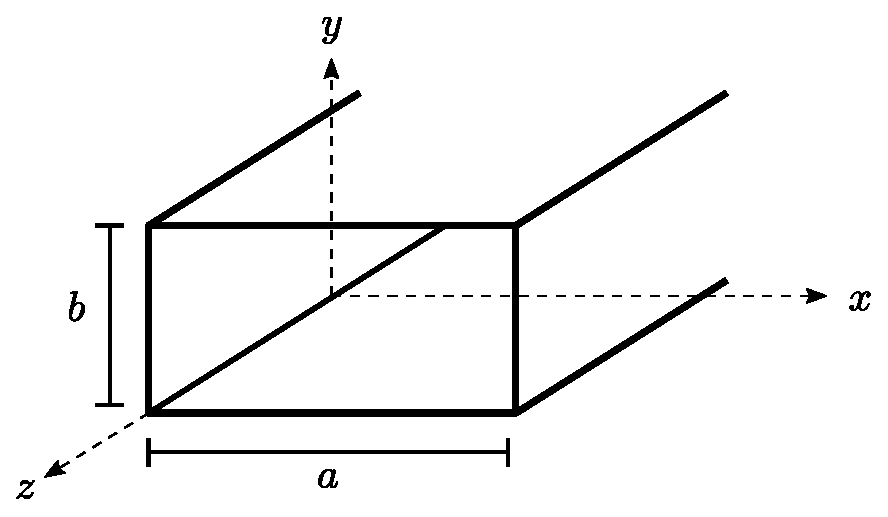
\includegraphics[width=1.0\columnwidth]{modules/m0223_fRectWG.eps} 
% https://commons.wikimedia.org/wiki ...
}}{An x-y-z coordinate system with x horizontal, y vertical, and z out of the page. Rectangular structure with cross section width a in the x dimension and b in the y dimension.}
\end{center}
%\centerline{\scriptsize 
%\copyright~\hyperref[m0223_fParallelPlateWaveguide_Credit]{C.\ Wang} 
%\href{https://creativecommons.org/licenses/by-sa/4.0/}{CC BY-SA 4.0} 
%} % \centerline 
\caption{
\label{m0223_fRectangularWaveguide}
Geometry for analysis of fields in a rectangular waveguide.
}
\end{figure}

Let us limit our attention to a region within the waveguide which is free of sources.
Expressed in phasor form, the electric field intensity within the waveguide is governed by the wave equation
%
\begin{equation}
\nabla^2 \widetilde{\bf E} + \beta^2 \widetilde{\bf E} = 0
\label{m0223_eWE}
\end{equation} 
%
where
%
\begin{equation}
\beta = \omega \sqrt{\mu \epsilon}
\end{equation}
%
Equation~\ref{m0223_eWE} is a partial differential equation.
This equation, combined with boundary conditions imposed by the perfectly-conducting plates, is sufficient to determine a unique solution.
This solution is most easily determined in Cartesian coordinates, as we shall now demonstrate.
First we express $\widetilde{\bf E}$ in Cartesian coordinates:
%
\begin{equation}
\widetilde{\bf E} = \hat{\bf x}\widetilde{E}_x + \hat{\bf y}\widetilde{E}_y + \hat{\bf z}\widetilde{E}_z
\label{m0223_eE}
\end{equation}
%
This facilitates the decomposition of Equation~\ref{m0223_eWE} into separate equations governing the $\hat{\bf x}$, $\hat{\bf y}$, and $\hat{\bf z}$ components of $\widetilde{\bf E}$:
%
\begin{flalign}
\nabla^2 \widetilde{E}_x + \beta^2 \widetilde{E}_x &= 0 \\
\nabla^2 \widetilde{E}_y + \beta^2 \widetilde{E}_y &= 0 \\
\nabla^2 \widetilde{E}_z + \beta^2 \widetilde{E}_z &= 0 
\end{flalign} 

Next we observe that the operator $\nabla^2$ may be expressed in Cartesian coordinates as follows:
%
\begin{equation}
\nabla^2 = \frac{\partial^2}{\partial x^2} + \frac{\partial^2}{\partial y^2} + \frac{\partial^2}{\partial z^2} 
\end{equation}
%
so the equations governing the Cartesian components of $\widetilde{\bf E}$ may be written as follows:
%
\begin{flalign}
\frac{\partial^2}{\partial x^2}\widetilde{E}_x + \frac{\partial^2}{\partial y^2}\widetilde{E}_x + \frac{\partial^2}{\partial z^2}\widetilde{E}_x + \beta^2 \widetilde{E}_x &= 0 \label{m0223_eEfx} \\
\frac{\partial^2}{\partial x^2}\widetilde{E}_y + \frac{\partial^2}{\partial y^2}\widetilde{E}_y + \frac{\partial^2}{\partial z^2}\widetilde{E}_y + \beta^2 \widetilde{E}_y &= 0 \label{m0223_eEfy} \\
\frac{\partial^2}{\partial x^2}\widetilde{E}_z + \frac{\partial^2}{\partial y^2}\widetilde{E}_z + \frac{\partial^2}{\partial z^2}\widetilde{E}_z + \beta^2 \widetilde{E}_z &= 0 \label{m0223_eEfz} 
\end{flalign} 

In general, we expect the total field in the waveguide to consist of unidirectional waves propagating in the $+\hat{\bf z}$ and $-\hat{\bf z}$ directions. 
We may analyze either of these waves; then the other wave is easily derived via symmetry, and the total field is simply a linear combination (superposition)
\index{superposition}
of these waves.
With this in mind, we limit our focus to the wave propagating in the $+\hat{\bf z}$ direction.

In Section~\ref{m0222_General_Relationships_Unidirectional_Waves}, 
%(``General Relationships for Unidirectional Waves'') 
it is shown that all components of the electric and magnetic fields can be easily calculated once $\widetilde{E}_z$ and $\widetilde{H}_z$ are known.  
The problem is further simplified by decomposing the unidirectional wave into TM and TE components.  
In this decomposition, the TM component is defined by the property that $\widetilde{H}_z=0$; i.e., is transverse (perpendicular) to the direction of propagation.
Thus, the TM component is completely determined by $\widetilde{E}_z$. 
Equations~\ref{m0222_eExu}--\ref{m0222_eHyu} simplify to become:
%
\begin{flalign}
\widetilde{E}_x &= -j\frac{k_z      }{k_{\rho}^2} \frac{\partial \widetilde{E}_z}{\partial x} \label{m0223_eExu} \\
\widetilde{E}_y &= -j\frac{k_z      }{k_{\rho}^2} \frac{\partial \widetilde{E}_z}{\partial y} \label{m0223_eEyu} \\
\widetilde{H}_x &= +j\frac{\omega\mu}{k_{\rho}^2} \frac{\partial \widetilde{E}_z}{\partial y} \label{m0223_eHxu} \\
\widetilde{H}_y &= -j\frac{\omega\mu}{k_{\rho}^2} \frac{\partial \widetilde{E}_z}{\partial x} \label{m0223_eHyu} 
\end{flalign}
%
where 
%
\begin{equation}
k_{\rho}^2 \triangleq \beta^2 - k_z^2 \label{m0223_ekrho}
\end{equation}
%
and $k_z$ is the phase propagation constant; i.e., the wave is assumed to propagate according to $e^{-jk_z z}$.

Now let us address the problem of finding $\widetilde{E}_z$, which will then completely determine the TM field.  As in Section~\ref{m0222_General_Relationships_Unidirectional_Waves}, we recognize that $\widetilde{E}_z$ can be represented as the propagation factor $e^{-jk_z z}$ times a factor that describes variation with respect to the remaining spatial dimensions $x$ and $y$:
%
\begin{equation}
\widetilde{E}_z = \widetilde{e}_z(x,y) e^{-jk_z z} 
\end{equation}
%
Substitution of this expression into Equation~\ref{m0223_eEfz} and dividing out the common factor of $e^{-jk_z z}$ yields:
%
\begin{equation}
\frac{\partial^2}{\partial x^2}\widetilde{e}_z + \frac{\partial^2}{\partial y^2}\widetilde{e}_z - k_z^2 \widetilde{e}_z + \beta^2 \widetilde{e}_z = 0
\end{equation}
%
The last two terms may be combined using Equation~\ref{m0223_ekrho}, yielding:
%
\begin{equation}
\frac{\partial^2}{\partial x^2}\widetilde{e}_z + \frac{\partial^2}{\partial y^2}\widetilde{e}_z + k_{\rho}^2 \widetilde{e}_z = 0 \label{m0223_eDE1}
\end{equation}
%
This is a partial differential equation for $\widetilde{e}_z$ in the variables $x$ and $y$.
This equation may be solved using the technique of \emph{separation of variables}.
\index{separation of variables}
In this technique, we recognize that $\widetilde{e}_z(x,y)$ can be written as the product of a function $X(x)$ which depends only on $x$, and a function $Y(y)$ that depends only on $y$.
That is,
%
\begin{equation}
\widetilde{e}_z(x,y) = X(x) Y(y)
\end{equation}
%
Substituting this expression into Equation~\ref{m0223_eDE1}, we obtain:
%
\begin{equation}
Y\frac{\partial^2}{\partial x^2}X + X\frac{\partial^2}{\partial y^2}Y + k_{\rho}^2 XY = 0 \label{m0223_eDE2}
\end{equation}
%
Next dividing through by $XY$, we obtain:
%
\begin{equation}
\frac{1}{X}\frac{\partial^2}{\partial x^2}X + \frac{1}{Y}\frac{\partial^2}{\partial y^2}Y + k_{\rho}^2 = 0 \label{m0223_eDE3}
\end{equation}
%
Note that the first term depends only on $x$, the second term depends only on $y$, and the remaining term is a constant.
Therefore, the sum of the first and second terms is a constant; namely $-k_{\rho}^2$.
Since these terms depend on either $x$ or $y$, and not both, the first term must equal some constant, the second term must equal some constant, and these constants must sum to $-k_{\rho}^2$.
Therefore, we are justified in separating the equation into two equations as follows:
%
\begin{flalign}
\frac{1}{X}\frac{\partial^2}{\partial x^2}X + k_x^2 &= 0 \label{m0223_eDE4x} \\
\frac{1}{Y}\frac{\partial^2}{\partial y^2}Y + k_y^2 &= 0 \label{m0223_eDE4y}
\end{flalign}
%
where the new constants $k_x^2$ and $k_y^2$ must satisfy
%
\begin{equation}
k_x^2+k_y^2 = k_{\rho}^2
\end{equation}
%
Now multiplying Equations~\ref{m0223_eDE4x} and \ref{m0223_eDE4y} by $X$ and $Y$, respectively, we find:
%
\begin{flalign}
\frac{\partial^2}{\partial x^2}X + k_x^2 X &= 0 \label{m0223_eDE5x} \\
\frac{\partial^2}{\partial y^2}Y + k_y^2 Y &= 0 \label{m0223_eDE5y}
\end{flalign}
%
These are familiar one-dimensional differential equations.  The solutions are:\footnote{Students are encouraged to confirm that these are correct by confirming that they are solutions to Equations~\ref{m0223_eDE5x} and \ref{m0223_eDE5x}, respectively.}
%
\begin{flalign}
X &= A\cos\left(k_x x\right) + B\sin\left(k_x x\right) \label{m0223_eX} \\
Y &= C\cos\left(k_y y\right) + D\sin\left(k_y y\right) \label{m0223_eY}
\end{flalign}
%
where $A$, $B$, $C$, and $D$ -- like $k_x$ and $k_y$ -- are constants to be determined.  
At this point, we observe that the wave we seek can be expressed as follows:
%
\begin{flalign}
\widetilde{E}_z &= \widetilde{e}_z(x,y) e^{-jk_z z} \nonumber \\
                &= X(x)~Y(y)~e^{-jk_z z} \label{m0223_eEzXYz} 
\end{flalign}
%
The solution is essentially complete except for the values of the constants $A$, $B$, $C$, $D$, $k_x$, and $k_y$.
The values of these constants are determined by applying the relevant electromagnetic boundary condition.
In this case, it is required that the component of $\widetilde{\bf E}$ that is tangent to a perfectly-conducting wall must be zero.
Note that the $\hat{\bf z}$ component of $\widetilde{\bf E}$ is tangent to all four walls; therefore:
%
\begin{flalign}
\widetilde{E}_z\left(x=0\right) &= 0 \\
\widetilde{E}_z\left(x=a\right) &= 0 \\
\widetilde{E}_z\left(y=0\right) &= 0 \\
\widetilde{E}_z\left(y=b\right) &= 0 
\end{flalign}
%
Referring to Equation~\ref{m0223_eEzXYz}, these boundary conditions in turn require:
%
\begin{flalign}
X\left(x=0\right) &= 0 \\
X\left(x=a\right) &= 0 \\
Y\left(y=0\right) &= 0 \\
Y\left(y=b\right) &= 0 
\end{flalign}
%
Evaluating these conditions using Equations~\ref{m0223_eX} and \ref{m0223_eY} yields:
%
\begin{flalign}
A\cdot 1                + B\cdot 0                  &= 0 \label{m0223_eXbc1} \\
A\cos\left(k_x a\right) + B\sin\left(k_x a\right)   &= 0 \label{m0223_eXbc2} \\
C\cdot 1                + D\cdot 0                  &= 0 \label{m0223_eYbc1} \\
C\cos\left(k_y b\right) + D\sin\left(k_y b\right)   &= 0 \label{m0223_eYbc2}
\end{flalign}
%
Equations~\ref{m0223_eXbc1} and \ref{m0223_eYbc1} can be satisfied only if $A=0$ and $C=0$, respectively.
Subsequently, Equations~\ref{m0223_eXbc2} and \ref{m0223_eYbc2} reduce to:
%
\begin{flalign}
\sin\left(k_x a\right)   &= 0 \label{m0223_eXbc2a}  \\
\sin\left(k_y b\right)   &= 0 \label{m0223_eYbc2a} 
\end{flalign}
%
This in turn requires:
%
\begin{flalign}
k_x &= \frac{m\pi}{a}~, ~~~ m=0, 1, 2 ... \label{m0223_ekxm}\\
k_y &= \frac{n\pi}{b}~, ~~~ n=0, 1, 2 ... \label{m0223_ekyn}
\end{flalign}
%
Each positive integer value of $m$ and $n$ leads to a valid expression for $\widetilde{E}_z$ known as a \emph{mode}.
\index{mode}
Solutions for which $m=0$ or $n=0$ yield $k_x=0$ or $k_y=0$, respectively.  These correspond to zero-valued fields, and therefore are not of interest.
The most general expression for $\widetilde{E}_z$ must account for all non-trivial modes.
Summarizing:
%
\begin{equation}
\widetilde{E}_z = \sum_{m=1}^{\infty} \sum_{n=1}^{\infty} \widetilde{E}_z^{(m,n)} \label{m0223_eEzTMall}
\end{equation}
%
where
 %
\begin{equation}
\widetilde{E}_z^{(m,n)} \triangleq E_0^{(m,n)} \sin\left(\frac{m\pi}{a} x\right) \sin\left(\frac{n\pi}{b} y\right) e^{-jk_z^{(m,n)} z} \label{m0223_eEzTM}
\end{equation}
%
where 
$E_0^{(m,n)}$ is an arbitrary constant (consolidating the constants $B$ and $D$), 
and,
since $k_x^2 + k_y^2 = k_{\rho}^2 \triangleq \beta^2-k_z^2$:
% 
\begin{equation}
k_z^{(m,n)} = \sqrt{ \omega^2\mu\epsilon - \left(\frac{m\pi}{a}\right)^2 - \left(\frac{n\pi}{b}\right)^2   } \label{m0223_ekzm}
\end{equation}

Summarizing:
%
%%%%%%%%%%%%%%%%%%%%%%%%%%%%%%%%%%%%%%%%%%%%%%%
%ORB HIGHLIGHT
\begin{mdframed}[backgroundcolor=yellow!20,nobreak=true] 
The TM ($\widetilde{H}_z=0$) component of the unidirectional ($+\hat{\bf z}$-traveling) wave in a rectangular waveguide is completely determined by Equation~\ref{m0223_eEzTMall}, and consists of modes as defined by Equations~\ref{m0223_eEzTM}, \ref{m0223_ekzm}, \ref{m0223_ekxm}, and \ref{m0223_ekyn}.  The remaining non-zero field components can be determined using Equations~\ref{m0223_eExu}--\ref{m0223_eHyu}.
\end{mdframed}
%%%%%%%%%%%%%%%%%%%%%%%%%%%%%%%%%%%%%%%%%%%%%%%

It is customary and convenient to refer to the TM modes in a rectangular waveguide using the notation ``TM$_{mn}$.''
For example, the mode TM$_{12}$ is given by Equation~\ref {m0223_eEzTM} with $m=1$ and $n=2$.

Finally, note that values of $k_z^{(m,n)}$ obtained from Equation~\ref{m0223_ekzm} are not necessarily real-valued.  
It is apparent that for any given value of $m$, $k_z^{(m,n)}$ will be imaginary-valued for all values of $n$ greater than some value.
Similarly, 
it is apparent that for any given value of $n$, $k_z^{(m,n)}$ will be imaginary-valued for all values of $m$ greater than some value.
This phenomenon is common to both TM and TE components, and so is addressed in a separate section (Section~\ref{m0224_Rectangular_Waveguide_Prop}).

%%%%%%%%%%%%%%%%%%%%%

{\bf Additional Reading:}
\begin{itemize}
\item ``\href{https://en.wikipedia.org/wiki/Waveguide_(radio_frequency)}{Waveguide (radio frequency)}'' on Wikipedia.
\item ``\href{https://en.wikipedia.org/wiki/Separation_of_variables}{Separation of variables}'' on Wikipedia.
\end{itemize}

\index{waveguide!rectangular|)}
\index{transverse magnetic|)}


